\documentclass[11pt]{exam}
\usepackage[T1]{fontenc}
\usepackage[amsthm]{newpx}
\usepackage[margin=1in]{geometry}
\usepackage{mathtools}
\usepackage{float}
\usepackage{enumerate}
\usepackage{listings}
\usepackage{hyperref}
\usepackage[boxed]{algorithm}
\usepackage[noend]{algpseudocode}
\hypersetup{
    colorlinks=true,
    linkcolor=blue,
    filecolor=magenta,      
    urlcolor=cyan,
}

% in order to compile this file you need to get 'header.tex' from
% Canvas and change the line below to the appropriate file path
%%% theorems

\theoremstyle{plain}            % following are "theorem" style
\newtheorem{theorem}{Theorem}[section]
\newtheorem{lemma}[theorem]{Lemma}
\newtheorem{corollary}[theorem]{Corollary}
\newtheorem{proposition}[theorem]{Proposition}
\newtheorem{claim}[theorem]{Claim}
\newtheorem{fact}[theorem]{Fact}
\newtheorem{openproblem}[theorem]{Open Problem}

\theoremstyle{definition}       % following are def style
\newtheorem{definition}[theorem]{Definition}
\newtheorem{conjecture}[theorem]{Conjecture}
\newtheorem{example}[theorem]{Example}
\newtheorem{protocol}[theorem]{Protocol}
\newtheorem{exercise}[theorem]{Exercise}

\theoremstyle{remark}           % following are remark style
\newtheorem{remark}[theorem]{Remark}
\newtheorem{note}[theorem]{Note}
%\newtheorem*{solution}{Solution}

%%% special sets
\newcommand{\bit}{\ensuremath{\{0,1\}}}
\newcommand{\bitt}{\ensuremath{\{-1,1\}}}
\newcommand{\ball}{\ensuremath{\mathcal{B}}}
\newcommand{\sph}{\ensuremath{\mathbb{S}}}
\newcommand{\odisc}[2]{\ensuremath{D(#1, #2)}}
\newcommand{\cdisc}[2]{\ensuremath{\bar{D}(#1, #2)}}
\newcommand{\emp}{\varnothing}

% constants
\newcommand{\E}{\ensuremath{\mathrm{e}}}
\newcommand{\I}{\ensuremath{\mathrm{i}}}
\newcommand{\Id}{\ensuremath{\mathrm{I}}}
\newcommand{\paulix}{\ensuremath{\mathrm{X}}}
\newcommand{\pauliy}{\ensuremath{\mathrm{Y}}}
\newcommand{\pauliz}{\ensuremath{\mathrm{Z}}}

% font for general-purpose algorithms
\newcommand{\algo}[1]{\ensuremath{\mathsf{#1}}}
% font for general-purpose computational problems
\newcommand{\problem}[1]{\ensuremath{\mathsf{#1}}}
% font for complexity classes
\newcommand{\class}[1]{\ensuremath{\mathsf{#1}}}

% asymptotics
\DeclareMathOperator{\poly}{poly}
\DeclareMathOperator{\polylog}{polylog}
\DeclareMathOperator{\negl}{negl}
\DeclareMathOperator{\bigO}{O}
\DeclareMathOperator{\litO}{o}
\DeclareMathOperator{\Otil}{\tilde{O}}
\DeclareMathOperator{\Ostar}{O^*}

%%% "LEFT-RIGHT" PAIRS OF SYMBOLS

% inner product
\DeclarePairedDelimiter\inner{\langle}{\rangle}
% absolute value
\DeclarePairedDelimiter\abs{\lvert}{\rvert}
% a set
\DeclarePairedDelimiter\set{\{}{\}}
% parens
\DeclarePairedDelimiter\parens{(}{)}
% tuple, alias for parens
\DeclarePairedDelimiter\tuple{(}{)}
% square brackets
\DeclarePairedDelimiter\bracks{[}{]}
% rounding off
\DeclarePairedDelimiter\round{\lfloor}{\rceil}
% floor function
\DeclarePairedDelimiter\floor{\lfloor}{\rfloor}
% ceiling function
\DeclarePairedDelimiter\ceil{\lceil}{\rceil}
% length of some vector, element
\DeclarePairedDelimiter\length{\lVert}{\rVert}
% "lifting" of a residue class
\DeclarePairedDelimiter\lift{\llbracket}{\rrbracket}
\DeclarePairedDelimiter\len{\lvert}{\rvert}
% bra-kets
\DeclarePairedDelimiter\bra{\langle}{\rvert}
\DeclarePairedDelimiter\ket{\lvert}{\rangle}
\newcommand{\braket}[2]{\ensuremath{\langle #1 \vert #2 \rangle}}
\newcommand{\ketbra}[2]{\ensuremath{\lvert #1 \rangle \langle #2 \rvert}}

%%% spacing

\newcommand{\ws}{\hspace{1pt}}
\newcommand{\wws}{\hspace{2pt}}
\newcommand{\hs}{\hspace{4pt}}
\newcommand{\hhs}{\hspace{8pt}}
\newcommand{\hhhs}{\hspace{12pt}}

%%% LISTS

\newcommand{\oneto}{1, \ldots,}
\newcommand{\onetop}{1 \cdots,}
\newcommand{\zeroto}{0, \ldots,}
\newcommand{\zerotop}{0 \cdots,}
\newcommand{\perm}[1]{\mathbf{(#1)}}
\newcommand{\permv}[1]{(#1)}
\newcommand{\varind}[2]{#1_1, \ldots, #1_#2}
\newcommand{\varindz}[2]{#1_0, \ldots, #1_#2}
\newcommand{\varindp}[2]{#1_1 \cdots #1_#2}
\newcommand{\varindpz}[2]{#1_0 \cdots #1_#2}
\newcommand{\seq}[2]{(#1_#2)_{#2=1}^\infty}
\newcommand{\seqz}[2]{(#1_#2)_{#2=0}^\infty}

%%% MATH OPERATORS

%\DeclareMathOperator{\pr}{\mathbf{P}}
%\DeclareMathOperator{\ex}{\mathbf{E}}
\DeclareMathOperator{\pr}{P}
\DeclareMathOperator{\ex}{E}
\DeclareMathOperator{\Span}{Span}
\DeclareMathOperator{\tr}{Tr}
\DeclareMathOperator{\supp}{Supp}
\DeclareMathOperator{\im}{Im}
\DeclareMathOperator{\var}{var}
\DeclareMathOperator{\vol}{vol}
\DeclareMathOperator{\sign}{sign}
\DeclareMathOperator{\dkl}{D_{KL}}
\DeclareMathOperator{\entr}{H}
\DeclareMathOperator{\fid}{F}
\DeclareMathOperator{\dist}{D}
\DeclareMathOperator{\ad}{ad}

% hats

\newcommand{\fhat}{\ensuremath{\hat{f}}}
\newcommand{\phat}{\ensuremath{\hat{p}}}
\newcommand{\that}{\ensuremath{\hat{t}}}

%%% BLACKBOARD SYMBOLS

\newcommand{\C}{\ensuremath{\mathbb{C}}}
\newcommand{\D}{\ensuremath{\mathbb{D}}}
\newcommand{\F}{\ensuremath{\mathbb{F}}}
\newcommand{\G}{\ensuremath{\mathbb{G}}}
\newcommand{\J}{\ensuremath{\mathbb{J}}}
\newcommand{\N}{\ensuremath{\mathbb{N}}}
\newcommand{\Q}{\ensuremath{\mathbb{Q}}}
\newcommand{\R}{\ensuremath{\mathbb{R}}}
\newcommand{\T}{\ensuremath{\mathbb{T}}}
\newcommand{\Z}{\ensuremath{\mathbb{Z}}}
\newcommand{\QR}{\ensuremath{\mathbb{QR}}}

% sets in calligraphic type

\newcommand{\calD}{\ensuremath{\mathcal{D}}}
\newcommand{\calF}{\ensuremath{\mathcal{F}}}
\newcommand{\calG}{\ensuremath{\mathcal{G}}}
\newcommand{\calH}{\ensuremath{\mathcal{H}}}
\newcommand{\calI}{\ensuremath{\mathcal{I}}}
\newcommand{\calL}{\ensuremath{\mathcal{L}}}
\newcommand{\calN}{\ensuremath{\mathcal{N}}}
\newcommand{\calP}{\ensuremath{\mathcal{P}}}
\newcommand{\calS}{\ensuremath{\mathcal{S}}}
\newcommand{\calX}{\ensuremath{\mathcal{X}}}
\newcommand{\calY}{\ensuremath{\mathcal{Y}}}

% matrices and vectors

\newcommand{\matA}{\ensuremath{\mathbf{A}}}
\newcommand{\matB}{\ensuremath{\mathbf{B}}}
\newcommand{\matC}{\ensuremath{\mathbf{C}}}
\newcommand{\matD}{\ensuremath{\mathbf{D}}}
\newcommand{\matE}{\ensuremath{\mathbf{E}}}
\newcommand{\matF}{\ensuremath{\mathbf{F}}}
\newcommand{\matG}{\ensuremath{\mathbf{G}}}
\newcommand{\matH}{\ensuremath{\mathbf{H}}}
\newcommand{\matI}{\ensuremath{\mathbf{I}}}
\newcommand{\matJ}{\ensuremath{\mathbf{J}}}
\newcommand{\matK}{\ensuremath{\mathbf{K}}}
\newcommand{\matL}{\ensuremath{\mathbf{L}}}
\newcommand{\matM}{\ensuremath{\mathbf{M}}}
\newcommand{\matN}{\ensuremath{\mathbf{N}}}
\newcommand{\matO}{\ensuremath{\mathbf{O}}}
\newcommand{\matP}{\ensuremath{\mathbf{P}}}
\newcommand{\matQ}{\ensuremath{\mathbf{Q}}}
\newcommand{\matR}{\ensuremath{\mathbf{R}}}
\newcommand{\matS}{\ensuremath{\mathbf{S}}}
\newcommand{\matT}{\ensuremath{\mathbf{T}}}
\newcommand{\matU}{\ensuremath{\mathbf{U}}}
\newcommand{\matV}{\ensuremath{\mathbf{V}}}
\newcommand{\matW}{\ensuremath{\mathbf{W}}}
\newcommand{\matX}{\ensuremath{\mathbf{X}}}
\newcommand{\matY}{\ensuremath{\mathbf{Y}}}
\newcommand{\matZ}{\ensuremath{\mathbf{Z}}}
\newcommand{\matzero}{\ensuremath{\mathbf{0}}}

\newcommand{\veca}{\ensuremath{\mathbf{a}}}
\newcommand{\vecb}{\ensuremath{\mathbf{b}}}
\newcommand{\vecc}{\ensuremath{\mathbf{c}}}
\newcommand{\vecd}{\ensuremath{\mathbf{d}}}
\newcommand{\vece}{\ensuremath{\mathbf{e}}}
\newcommand{\vecf}{\ensuremath{\mathbf{f}}}
\newcommand{\vecg}{\ensuremath{\mathbf{g}}}
\newcommand{\vech}{\ensuremath{\mathbf{h}}}
\newcommand{\veck}{\ensuremath{\mathbf{k}}}
\newcommand{\vecm}{\ensuremath{\mathbf{m}}}
\newcommand{\vecp}{\ensuremath{\mathbf{p}}}
\newcommand{\vecq}{\ensuremath{\mathbf{q}}}
\newcommand{\vecr}{\ensuremath{\mathbf{r}}}
\newcommand{\vecs}{\ensuremath{\mathbf{s}}}
\newcommand{\vect}{\ensuremath{\mathbf{t}}}
\newcommand{\vecu}{\ensuremath{\mathbf{u}}}
\newcommand{\vecv}{\ensuremath{\mathbf{v}}}
\newcommand{\vecw}{\ensuremath{\mathbf{w}}}
\newcommand{\vecx}{\ensuremath{\mathbf{x}}}
\newcommand{\vecy}{\ensuremath{\mathbf{y}}}
\newcommand{\vecz}{\ensuremath{\mathbf{z}}}
\newcommand{\veczero}{\ensuremath{\mathbf{0}}}
\newcommand{\vecone}{\ensuremath{\mathbf{1}}}

\newcommand{\vecell}{\ensuremath{\boldsymbol\ell}}
\newcommand{\vecalpha}{\ensuremath{\boldsymbol\alpha}}
\newcommand{\vecbeta}{\ensuremath{\boldsymbol\beta}}
\newcommand{\veceta}{\ensuremath{\boldsymbol\eta}}
\newcommand{\vecmu}{\ensuremath{\boldsymbol\mu}}
\newcommand{\vecphi}{\ensuremath{\boldsymbol\phi}}
\newcommand{\vecsigma}{\ensuremath{\boldsymbol\sigma}}
\newcommand{\vectheta}{\ensuremath{\boldsymbol\theta}}
\newcommand{\vecxi}{\ensuremath{\boldsymbol\xi}}

%%% misc

\newcommand{\ind}{\ensuremath{\mathbf{1}}}

\newcommand{\congmod}[3]{#1 \equiv #2 \textrm{ modulo } #3}

\newcommand{\dee}{\,\mathrm{d}}
\newcommand{\de}{\mathrm{d}}
\newcommand{\dx}{\,\mathrm{d} x}

\newcommand{\ol}{\overline}
\newcommand{\inv}[1]{\ensuremath{#1^{-1}}}
\newcommand{\tsp}[1]{\ensuremath{#1^{\top}}}


\newcommand{\eps}{\varepsilon}
\newcommand{\ph}{\varphi}

\newcommand{\Ra}{\Rightarrow}
\newcommand{\Lra}{\Leftrightarrow}
\newcommand{\rsqa}{\rightsquigarrow}

\newcommand{\trl}{\triangleleft}
\newcommand{\trr}{\triangleright}

\newcommand{\func}[3]{#1: #2 \to #3}
\newcommand{\dd}[1]{\frac{\mathrm{d}}{\mathrm{d}#1}}
\newcommand{\ptl}[1]{\frac{\partial}{\partial #1}}
\newcommand{\prtl}[2]{\frac{\partial #1}{\partial #2}}

\newcommand{\matrixtt}[4]{
  \begin{pmatrix*}[r]
        #1 & #2 \\
        #3 & #4
    \end{pmatrix*}
}

%%% for homework and section notes

\newcommand{\commonheader}[2]{
    \pagestyle{headandfoot}
    \setlength{\headheight}{26pt}
    \setlength{\headsep}{16pt}

    \header
        {\small{\textbf{CSCI 3383: Algorithms}} \\ \footnotesize{\textbf{Boston College, Fall 2021}}}
        {#1}
        {#2}

    \firstpageheadrule
    \runningheadrule

    \footer
        {}
        {Page \thepage~of~\numpages}
        {}
}

\newcommand{\hwheader}{
    \commonheader
        {\Large \textbf{Homework \hwnum}}
        {\small \textbf{Due at \duedate}}
}

\newcommand{\hwslnheader}{
    \commonheader
    	{}
        {\Large \textbf{Solutions to Homework \hwnum}}
    \printanswers
}

\newcommand{\notesheader}{
    \commonheader
        {\Large \textbf{Section Notes \sectionnum}}
    	{}
}

\newcommand{\hwpreface}{
\noindent 
%Problems marked with \textbf{E} are graded on effort, which
%means that they are graded subjectively on the perceived effort %you
%put into them, rather than on correctness. 
We strongly encourage you
to typeset your solutions in \LaTeX. 
A typed assignment (in any word processing tool) will receive $5$ \textbf{extra} points (out of 100 for an assignment). For bonus questions, we will not provide any insight during office hours or Piazza, and we do not guarantee anything about the difficulty of these questions. 
\vspace{1ex}\\
If you collaborated with someone, you must state their names. You must write your \textbf{own} solution in your \textbf{own} words and \textbf{may not} look at any other student’s write-up.
}

\newcommand{\hint}[1]{
\emph{Hint}: #1
}

% for effort questions
\let\Eitem=\relax
\def\effortE{\textbf{E}~}
\makeatletter
\def\Eitem{%
    \expandafter\let\expandafter\originallabel\csname labelenum\romannumeral\@enumdepth\endcsname
    \expandafter\def\csname labelenum\romannumeral\@enumdepth\expandafter\endcsname\expandafter{%
        \expandafter\effortE\originallabel}%
    \item
    \expandafter\let\csname labelenum\romannumeral\@enumdepth\endcsname\originallabel
}
\makeatother

\allowdisplaybreaks



\begin{document}

\noindent {\bf \Large  Liam Murphy}\\

\noindent {\it \Large  Lecture Outline}\\

\section*{Outline}

\begin{itemize}

\item Start with general 2-3 minute talk about how the abstract algorithms we learn have pretty important uses, even for students (not just researchers)

\item Introduce the idea of a technical interview: explain how the skill the companies are looking for is not coding, it's knowledge of algorithms and data structures

\item Introduce the problem that we will be studying: the Knight's Path

\item (be sure to mention that this is totally {\it not} a problem from an actual interview)

\item Explain that while this big description of a problem seems scary at first glance, it's actually a fairly simple application of a common algorithm we saw in class, the BFS

\item Show how to translate the problem from words into a graph problem

\item Solve the problem (important: show pseudocode for it then maybe show a working python implementation ?? if I have time to code that up this week)

\item Closing remarks about how the hard part is translating the problem from words to an algorithmic problem that is easy to solve

\end{itemize}


\section*{Knight's Path}

{\large Description}\\
Given an $n\times n$ chess board, a starting position, and ending position,
and a bishop position, compute the shortest path a knight starting at the
start position and ending at the end position can take without being
threatened by the bishop. If the knight can capture the bishop, then
it is free to take any path.\\\\
{\large Notes}\\
A knight can move in an L-shape. That is, given some position $(p,q)$ on
the board, the knight can move to $(p+1,q+2), (p+2,q+1), (p-1,q+2)$, etc.
Here is a picture for better visualization.
\begin{figure}[H]
	\centering
	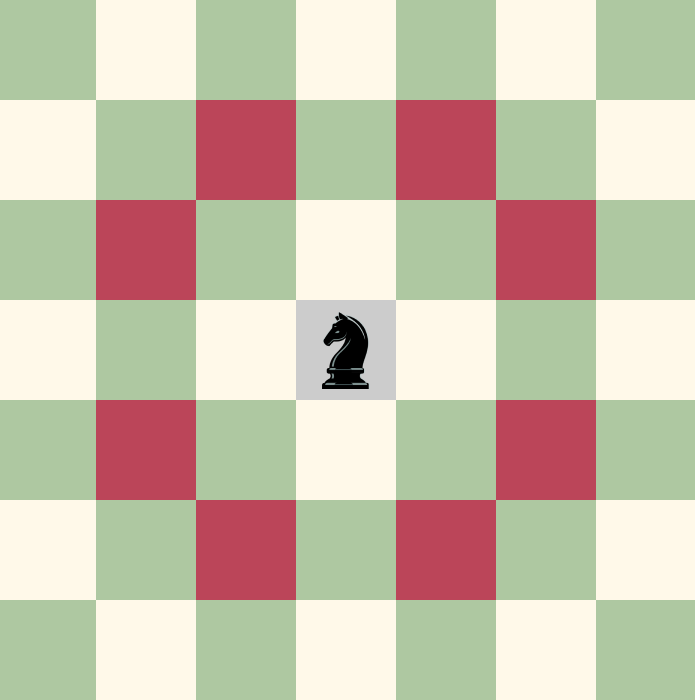
\includegraphics[width=\linewidth]{knight_moves.png}
	\caption{A knight's possible moves}
\end{figure}
The shortest path refers to the path that costs the knight the least
amount of moves. Now, the bishop moves in a diagonal pattern, so when
designing our algorithm, we cannot land on any spaces that are diagonal
from the bishop, unless we capture (land on top of it) first.
With the details now in mind, we're ready to start.

\newpage
\section*{Solution}
We want to design an algorithm that treats the chessboard as a graph, then use BFS to find the shortest path (with a few modifications, of course).
However, we can't just make the entire chessboard, a graph, because the
knight can't move to just any space! Here's the idea: use BFS to determine
how many moves it would take to reach the bishop, capture, then move to the
ending position (or if this is even possible) and compare it with just
avoiding the bishop's threat and going straight to the end position (if
this is even possible). Return the length of the shorter path, if either
answer reaches the end space.
\begin{algorithm}[H]
\begin{algorithmic}
\Procedure{Make-Node}{$x,y,d$}
	\Return{$(x,y,d)$}
\algorithmiccomment{{\it A Node is a 3-Tuple with an x coordinate, y coordinate, and integer distance}}
\EndProcedure
\Procedure{Is-Valid}{$x,y,n$}
	\If{$x<1$ or $y<1$ or $x>n$ or $y>n$}
		\Return{false}
	\EndIf
	\Return{true}
\EndProcedure
\Procedure{Is-Valid-Bishop}{$x,y,A$}
	\If{$(x,y)$ in $A$}
		\Return{false}
	\EndIf
	\Return{true}
\EndProcedure
\Procedure{Bishop-Positions}{$x,y,n$}
	\State{$A\gets\varnothing$}
	\For{$i\in\set{1,2,\ldots,n}$}
		\If{\Call{Is-Valid}{$x+i,y+i,n$}}
			\State{$A.add(x,y)$}
		\EndIf
		\If{\Call{Is-Valid}{$x-i,y+i,n$}}
			\State{$A.add(x,y)$}
		\EndIf
		\If{\Call{Is-Valid}{$x+i,y-i,n$}}
			\State{$A.add(x,y)$}
		\EndIf
		\If{\Call{Is-Valid}{$x-i,y-i,n$}}
			\State{$A.add(x,y)$}
		\EndIf
	\EndFor
	\Return{$A$}
\EndProcedure
\Procedure{Shortest-Path}{$x_0,y_0,x_1,y_1,n,b,A$}
\algorithmiccomment{{\it $x_0,y_0$ is start position, $x_1,y_1$ is end position, $n$ is dimension, and $b$ is a Boolean for if the bishop exists}}
	\State{$row\gets\set{2,2,-2,-2,1,1,-1,-1}$}
	\State{$col\gets\set{-1,1,1,-1,2,-2,2,-2}$}
	\State{$visited\gets\varnothing$}
	\State{Queue $Q\gets \{\Call{Make-Node}{x_0,y_0,0}\}$}
	\While{$Q\neq\varnothing$}
		\State{$v\gets Q.pop$}
		\If{$v.x=x_1$ and $v.y=y_1$}
			\Return{$v.d$}
		\EndIf
		\If{$v\notin visited$}
			\State{$visited.add(v)$}
			\For{$i\in\set{1,2,\ldots,8}$}
				\State{$x_{new}\gets v.x+col[i]$}
				\State{$y_{new}\gets v.y+row[i]$}
				\If{$b=true$}
					\If{\Call{Is-Valid}{$x_{new},y_{new},n$} and \Call{Is-Valid-Bishop}{$x_{new},y_{new},A$}}
						\State{$Q.add(\Call{Make-Node}{x_{new},y_{new},v.d+1})$}
					\EndIf
				\Else
					\If{\Call{Is-Valid}{$x_{new},y_{new},n$}}
						\State{$Q.add(\Call{Make-Node}{x_{new},y_{new},v.d+1})$}
					\EndIf
				\EndIf
			\EndFor
		\EndIf
	\EndWhile
	\Return{-1}
\EndProcedure
\Procedure{Knight's-Path}{$x_0,y_0,x_1,y_1,b_x,b_y,n$}
	\State{$A\gets$ \Call{Bishop-Positions}{$b_x,b_y,n$}}
	\State{to-bishop $\gets$ \Call{Shortest-Path}{$x_0,y_0,b_x,b_y,n,true,A$}}
	\State{to-goal $\gets$ \Call{Shortest-Path}{$x_0,y_0,x_1,y_1,n,true,A$}}
	\If{to-bishop $\neq -1$}
		\State{b-to-goal $\gets$ \Call{Shortest-Path}{$b_x,b_y,x_1,y_1,n,false,A$}}
		\If{b-to-goal $\neq -1$}
			\If{to-goal $\neq -1$}
				\Return{$\min(\text{to-bishop}+\text{b-to-goal},\text{to-goal})$}
			\Else 
				\Return{$\text{to-bishop}+\text{b-to-goal}$}
			\EndIf
		\Else 
			\Return{to-goal}
		\EndIf
	\Else 
		\Return{to-goal}
	\EndIf
\EndProcedure
\end{algorithmic}
\end{algorithm}
\end{document}
